\documentclass{article}
\usepackage[margin=1in]{geometry}
\usepackage{siunitx}
\usepackage{array}
\usepackage{booktabs}
\usepackage{hyperref}
\usepackage{graphicx}

\begin{document}
\author{Sachith Dunatunga}
\title{16.930 PS3}
\maketitle

\section{Convergence Study}
We used meshes where $m = n = [3, 4, 6, 8, 12]$.
We have plotted the results of the convergence study in \ref{fig:cc}.
The rates are shown in table \ref{tbl:cc}.
Despite using a small time step ($\Delta t = 0.001$), we didn't quite see the expected convergence rates.
In order to calculate the rates, we used only the last three points in both cases.
I suspect the temporal error is starting to limit the slope at larger grid sizes, as $p=2$ displays the correct behavior, but the slopes for $p = 3,4$ are a bit under what they should be.
Although not shown, meshes at size $m = n = 16$ had essentially the same error as the $m = n = 12$ case for the fourth order elements at this time step size.
Unfortunately, my residual evaluation code is quite slow and the largest cases already took more than an hour to run.
Switching to the given implementation did not seem to help much either with the speed, and I ran out of patience after multiple attempts.

\begin{figure}[!ht]
\centering
\begin{tabular}{c c}
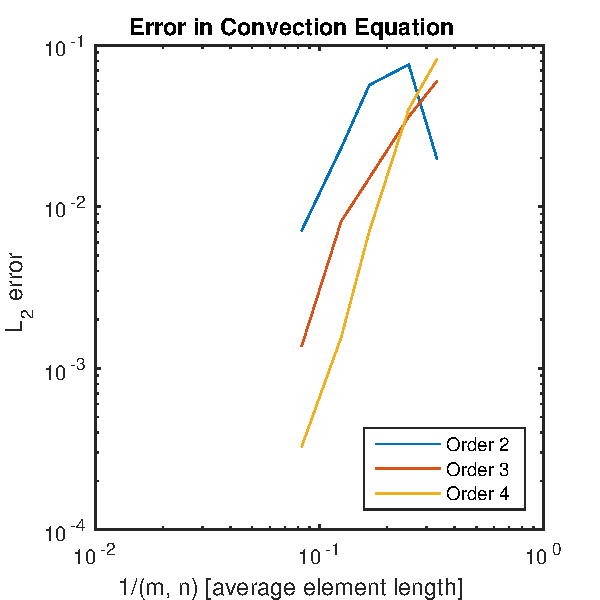
\includegraphics[scale=0.8]{cc_err_nodistort.pdf} &
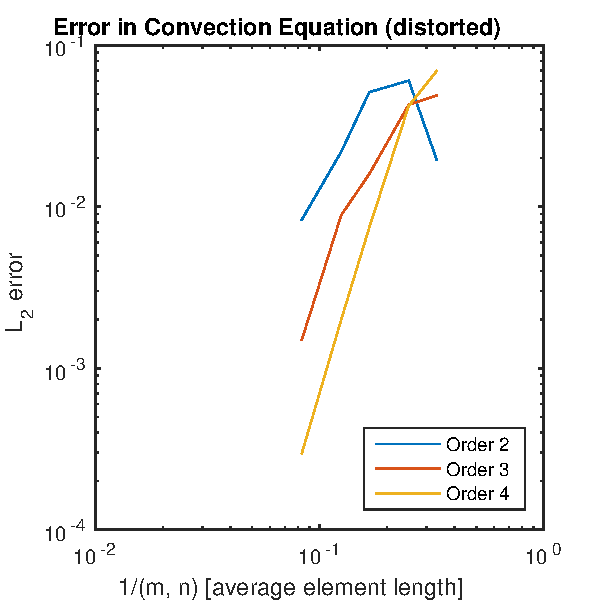
\includegraphics[scale=0.8]{cc_err_distort.pdf}
\end{tabular}
\caption{$L_2$ error for both the regular (left) and distorted (right) meshes. The second order elements converge as expected, but the higher order elements seem to be slightly underperforming. I am not sure if this is due to the temporal error. Rates are given in table \ref{tbl:cc}. The distortion does not seem to affect the rate much.}
\label{fig:cc}
\end{figure}

\begin{table}[!ht]
\centering
\caption{Table of convergence rates for regular and distorted elements.}
\label{tbl:cc}
\begin{tabular}{c c c}
Order & Regular & Distorted \\
\midrule
2 & 2.98247 & 2.61016\\
3 & 3.51268 & 3.47745 \\
4 & 4.38533 & 4.64987 \\
\end{tabular}
\end{table}

\section{rinvexpl.m Implementation}
Please see the code located at \texttt{2DG.3/dgker/myrinvexpl.m} in the zip file accompanying this report.
I have also submitted it separately on Stellar.

\section{Wave Equation}
From inspection, we see that if we have a grid with odd number of subdivisions n, the (n+1)/2 innermost concentric grid line goes through (e, 0).
We select all nodes which are close to this grid line and plot the magnitude of the scattered field versus their respective angles.
There are multiple values per choice of theta due to the fact that two or more DG elements meet at these points.

The meshes were given by 11 points in r and 20 points in theta (for p=3) and 21 points in r and 35 points in theta (for p=1).
This yields a similar number of DOFs.
Despite the similar number of DOFs, the simulation of the p=3 case took much less time.

I'm not sure if there is an error in my residual evaluation or something else, but the scattered field does not look very good (shown in figure \ref{fig:wave}).
The features are almost as I expect, but they are much noiser than I thought they would be.
The higher order elements seem to be doing a better job, but share the same type of problem.
I have reduced the time step size to see if this is due to the explicit integration, but the simulations are still running.

\begin{figure}[!ht]
\centering
\begin{tabular}{c c}
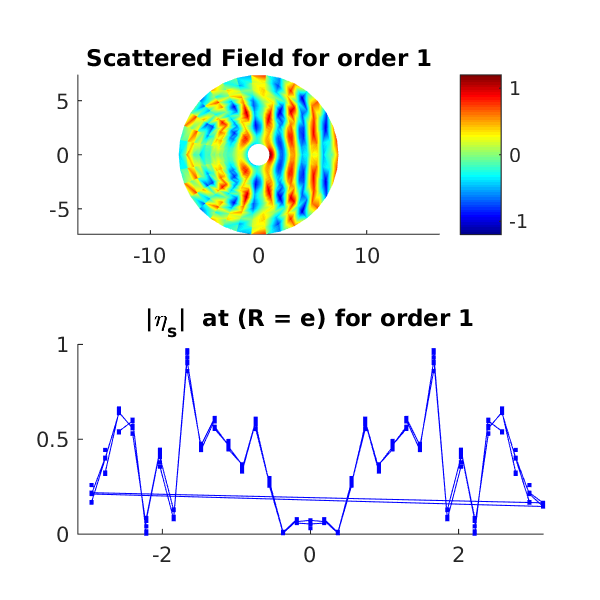
\includegraphics[scale=0.8]{wave_1.pdf} &
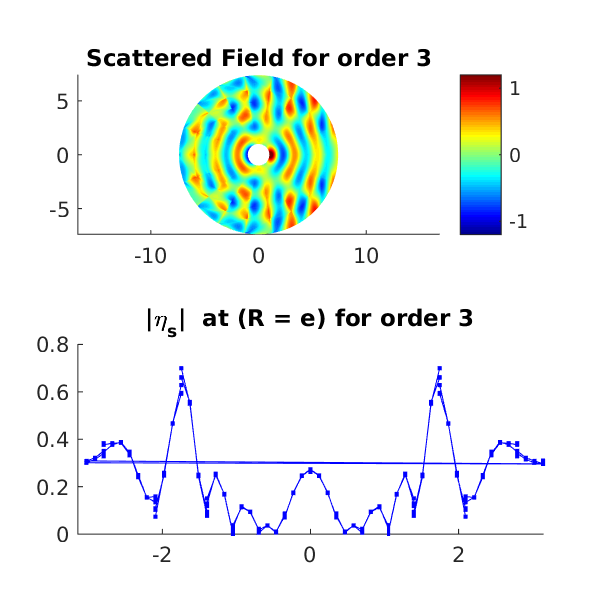
\includegraphics[scale=0.8]{wave_3.pdf}
\end{tabular}
\caption{The scattering of waves around a cylinder. The results are much noiser than I expected, but I am not sure what the reason for this is.}
\label{fig:wave}
\end{figure}

\section{Euler Equations}
I have not run these simulations yet; this will be updated if they can be completed in a reasonable time.

\section{Euler Equations with Obstacle}
The mach number and pressures are plotted for both the p=1 and p=3 cases in figure \ref{fig:channel-obs}.
The mesh for the p=1 case had 37x21 elements, while the p=3 case had 21x12 (this may be too low as indicated by the lack of boundary layer).
We see that the simulations look similar, although the mach number is lower on the downstream edge in the p=1 case.
However, the p=3 case took less time to compute, despite having a similar number of DOFs (I'm not sure if this is due to my implementation or not though).

\begin{figure}[!ht]
\centering
\begin{tabular}{c c}
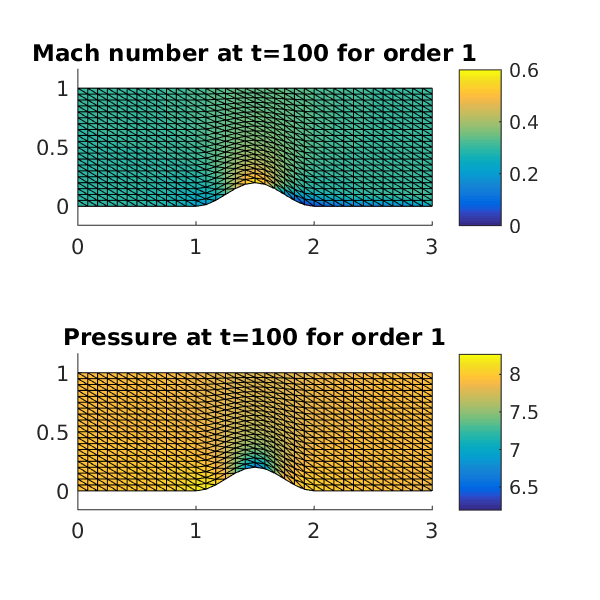
\includegraphics[scale=0.8]{channel_obs_1.pdf} &
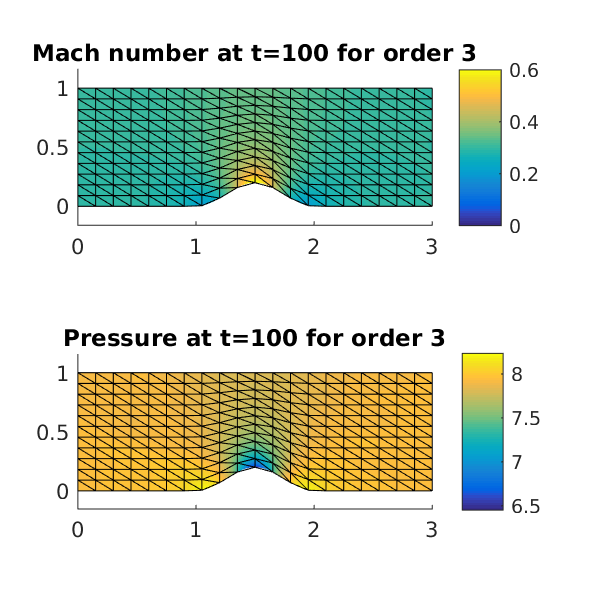
\includegraphics[scale=0.8]{channel_obs_3.pdf}
\end{tabular}
\caption{The Euler channel problem with two different meshes at p=1 and p=3. The number of DOFs are similar between the meshes.}
\label{fig:channel-obs}
\end{figure}

\end{document}
